
\actTitle{Worksheet 3.1}

\noindent \textbf{Instructions:}  Work together in groups of  3 or 4 to complete the following problems.

Student goals:
\begin{itemize}
\item Determine if a given function is one-to-one. The function can
  be given in graphical, tabular, or algebraic forms.
\item Explicitly show that a function is one-to-one or demonstrate why
  a function is not one-to-one.
\item Determine the inverse of a given function. The function can be
  given in tabular or algebraic forms.
\item Determine the domain and range of the inverse of a function. The
  function can be given in graphical, tabular, or algebraic forms.
\item Limit the domain of a function that is not one-to-one so that an
  inverse can be defined on the resulting restricted domain.
\end{itemize}


For the following set of questions your group should work with three
functions that you will construct. You will start with three basic
functions and transform them into new functions which will be used
throughout the remaining questions.
\begin{enumerate}
\item Use $g(x)=(x+1)^2$ and two of the following functions for your
  group.  Along with $g(x)$ choose two from the following functions:
  $$f(x)=x-1, \quad \quad
  h(x)=(x-2)^3, \quad \quad
  j(x)=\frac{1}{x}+1, \quad \quad
  m(x)=\sqrt{x+2}-1,  \quad \quad
  p(x)=\sqrt[3]{x}.$$

\item State the parent function for each of your three functions.

  \vfill

\item For each of your functions, briefly state the transformations
  that will change the parent function to the final function.

  \vfill

  \clearpage

\item Sketch the graphs of each of your functions on a separate axis
  below, and include the parent function of each function on the same
  axis.
  
  \begin{tabular}{p{0.5\linewidth}p{0.5\linewidth}}

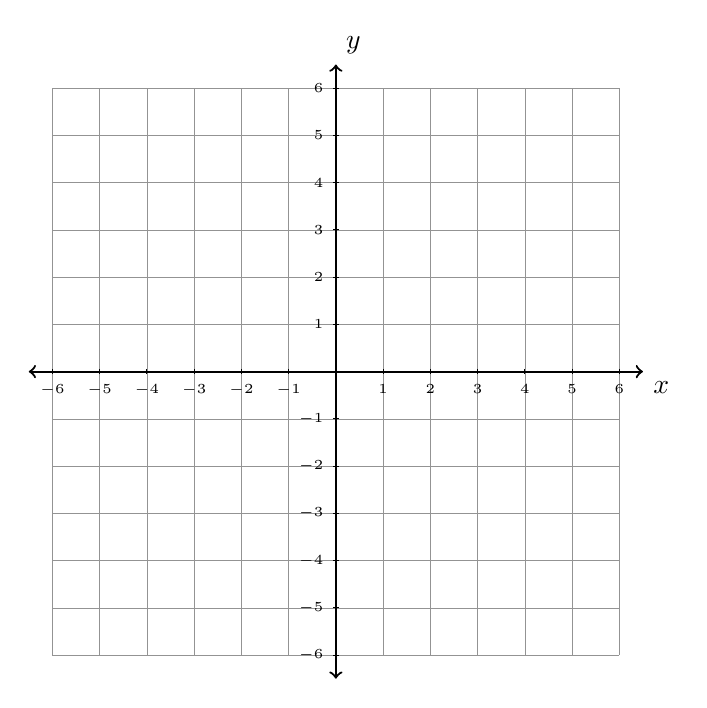
\begin{tikzpicture}[y=.6cm, x=.6cm,font=\sffamily,
	mydot/.style={
    circle,
    fill=white,
    draw,
    outer sep=0pt,
    inner sep=1.5pt
  }]
    %% Add a grid
    \draw[step = 1, gray, very thin,opacity=0.85] (-6, -6) grid (6, 6);
 	%% Draw the axes
	\draw[thick,<->] (-6.5,0) -- coordinate (x axis mid) (6.5,0) node[anchor = north west] {$x$};
    \draw[thick,<->] (0,-6.5) -- coordinate (y axis mid) (0,6.5) node[anchor = south west] {$y$};
    %% Label the y axis
    \foreach \y in {-6,...,-1,1,2,...,6} {
      \draw (1pt, \y) -- (-1pt, \y) node[anchor =  east] {\tiny$\y$};
    }
    %% Label the x axis
    \foreach \x in {-6,...,-1,1,2,...,6} {
      \draw (\x,1pt) -- (\x,-1pt) node[anchor = north] {\tiny$\x$};
    }

  \end{tikzpicture}

&


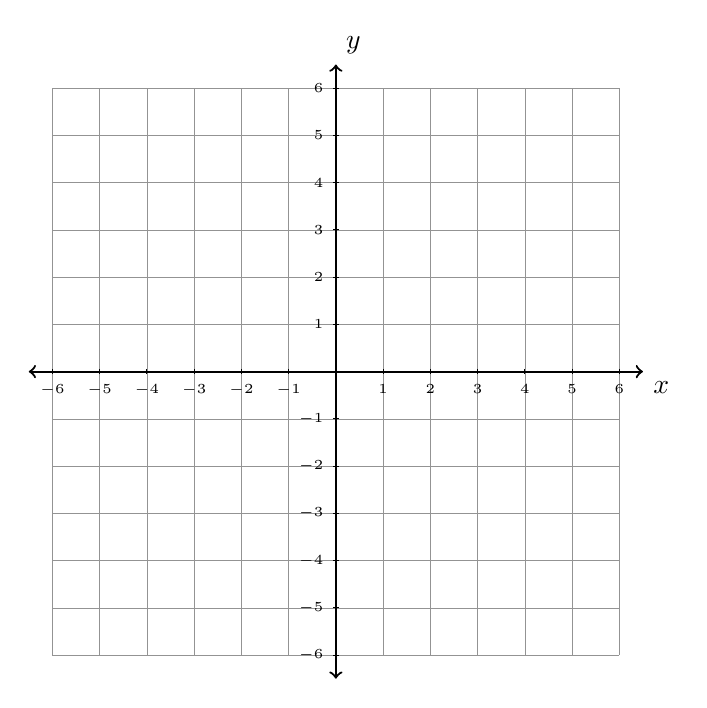
\begin{tikzpicture}[y=.6cm, x=.6cm,font=\sffamily,
	mydot/.style={
    circle,
    fill=white,
    draw,
    outer sep=0pt,
    inner sep=1.5pt
  }]
    %% Add a grid
    \draw[step = 1, gray, very thin,opacity=0.85] (-6, -6) grid (6, 6);
 	%% Draw the axes
	\draw[thick,<->] (-6.5,0) -- coordinate (x axis mid) (6.5,0) node[anchor = north west] {$x$};
    \draw[thick,<->] (0,-6.5) -- coordinate (y axis mid) (0,6.5) node[anchor = south west] {$y$};
    %% Label the y axis
    \foreach \y in {-6,...,-1,1,2,...,6} {
      \draw (1pt, \y) -- (-1pt, \y) node[anchor =  east] {\tiny$\y$};
    }
    %% Label the x axis
    \foreach \x in {-6,...,-1,1,2,...,6} {
      \draw (\x,1pt) -- (\x,-1pt) node[anchor = north] {\tiny$\x$};
    }

  \end{tikzpicture}

\\

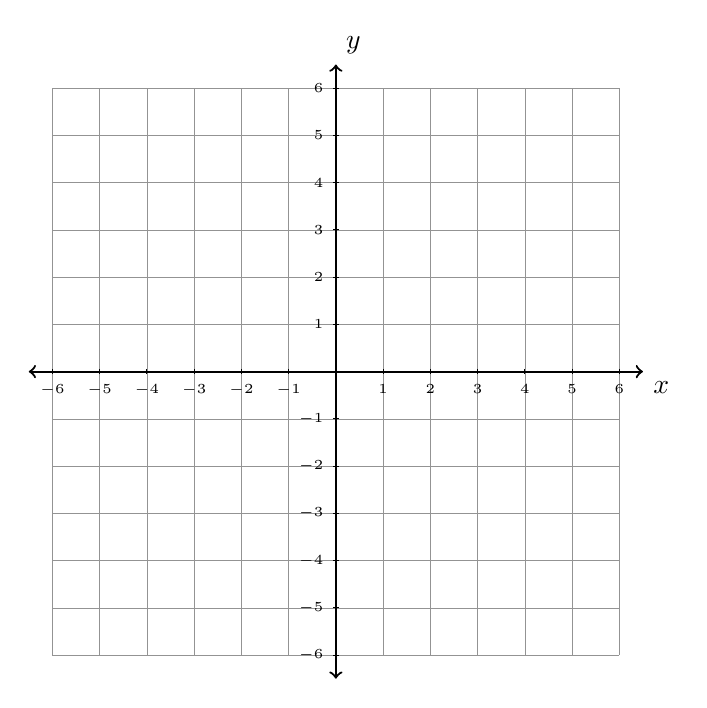
\begin{tikzpicture}[y=.6cm, x=.6cm,font=\sffamily,
	mydot/.style={
    circle,
    fill=white,
    draw,
    outer sep=0pt,
    inner sep=1.5pt
  }]
    %% Add a grid
    \draw[step = 1, gray, very thin,opacity=0.85] (-6, -6) grid (6, 6);
 	%% Draw the axes
	\draw[thick,<->] (-6.5,0) -- coordinate (x axis mid) (6.5,0) node[anchor = north west] {$x$};
    \draw[thick,<->] (0,-6.5) -- coordinate (y axis mid) (0,6.5) node[anchor = south west] {$y$};
    %% Label the y axis
    \foreach \y in {-6,...,-1,1,2,...,6} {
      \draw (1pt, \y) -- (-1pt, \y) node[anchor =  east] {\tiny$\y$};
    }
    %% Label the x axis
    \foreach \x in {-6,...,-1,1,2,...,6} {
      \draw (\x,1pt) -- (\x,-1pt) node[anchor = north] {\tiny$\x$};
    }

  \end{tikzpicture}
  

&


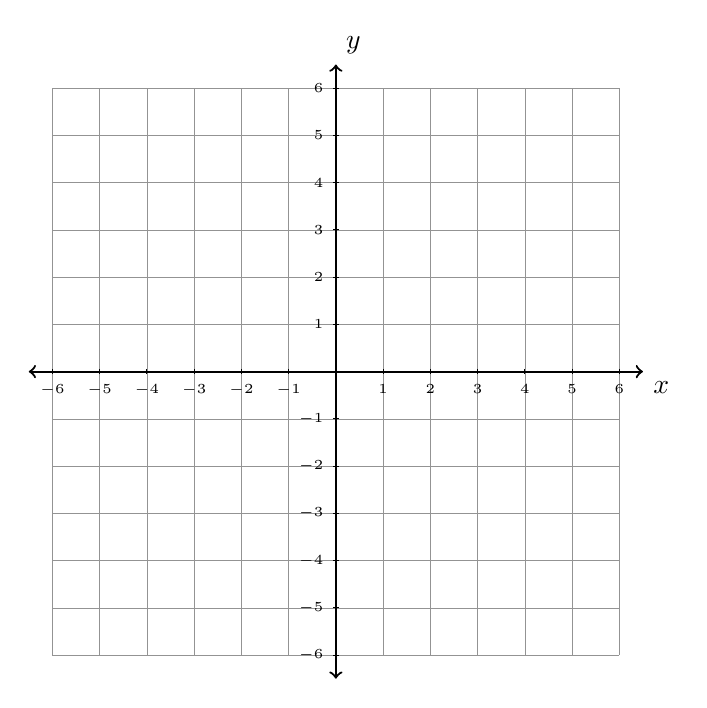
\begin{tikzpicture}[y=.6cm, x=.6cm,font=\sffamily,
	mydot/.style={
    circle,
    fill=white,
    draw,
    outer sep=0pt,
    inner sep=1.5pt
  }]
    %% Add a grid
    \draw[step = 1, gray, very thin,opacity=0.85] (-6, -6) grid (6, 6);
 	%% Draw the axes
	\draw[thick,<->] (-6.5,0) -- coordinate (x axis mid) (6.5,0) node[anchor = north west] {$x$};
    \draw[thick,<->] (0,-6.5) -- coordinate (y axis mid) (0,6.5) node[anchor = south west] {$y$};
    %% Label the y axis
    \foreach \y in {-6,...,-1,1,2,...,6} {
      \draw (1pt, \y) -- (-1pt, \y) node[anchor =  east] {\tiny$\y$};
    }
    %% Label the x axis
    \foreach \x in {-6,...,-1,1,2,...,6} {
      \draw (\x,1pt) -- (\x,-1pt) node[anchor = north] {\tiny$\x$};
    }

  \end{tikzpicture}
  
  
\end{tabular}


\item Calculate the domain and range for each of your three functions.

  \vfill

  \clearpage

\item Determine \emph{algebraically} if each of your functions are one-to-one.  

  \vfill
  \vfill

\item For each of your functions that are not one-to-one, make a
  domain restriction so that the function becomes one-to-one on the
  new domain.

\vfill

\clearpage

\item For each of your functions (including those with new domain restrictions), find their inverse functions.

\vfill

\item Use function composition to verify that the inverse functions you have described are truly inverses to your functions.

\vfill

\clearpage

\item Graph your function and its inverse on the same coordinate axes.  Check that they are properly symmetric to each other.

\begin{multicols}{2}

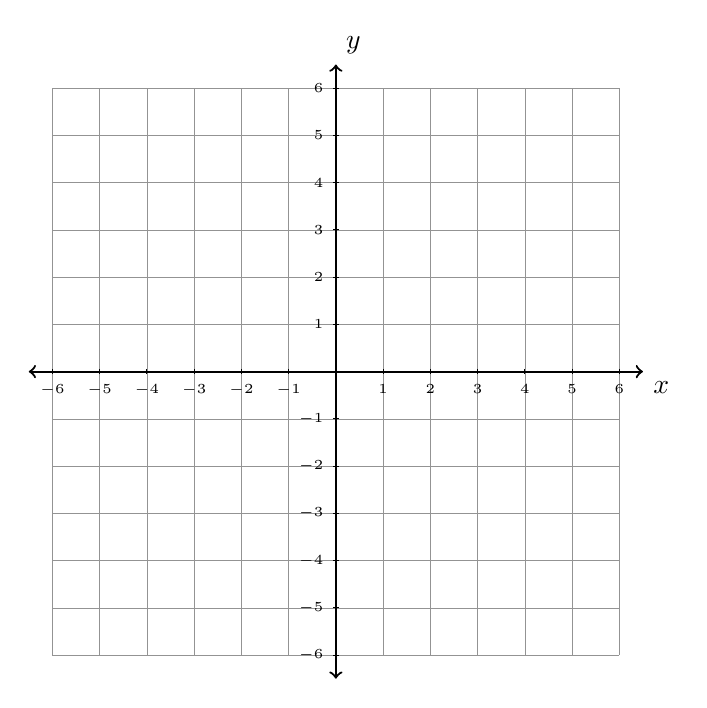
\begin{tikzpicture}[y=.6cm, x=.6cm,font=\sffamily,
	mydot/.style={
    circle,
    fill=white,
    draw,
    outer sep=0pt,
    inner sep=1.5pt
  }]
    %% Add a grid
    \draw[step = 1, gray, very thin,opacity=0.85] (-6, -6) grid (6, 6);
 	%% Draw the axes
	\draw[thick,<->] (-6.5,0) -- coordinate (x axis mid) (6.5,0) node[anchor = north west] {$x$};
    \draw[thick,<->] (0,-6.5) -- coordinate (y axis mid) (0,6.5) node[anchor = south west] {$y$};
    %% Label the y axis
    \foreach \y in {-6,...,-1,1,2,...,6} {
      \draw (1pt, \y) -- (-1pt, \y) node[anchor =  east] {\tiny$\y$};
    }
    %% Label the x axis
    \foreach \x in {-6,...,-1,1,2,...,6} {
      \draw (\x,1pt) -- (\x,-1pt) node[anchor = north] {\tiny$\x$};
    }
    %% Draw the function.
 %   \begin{scope}
 %        \draw[very thick,black] (-3,2) -- (1,1);
 %        \draw[very thick,black] (3.05,1.05) -- (4,3);
    %semi-circle
  %       \draw[very thick, black] (1,1) arc [radius=1, start angle=180, end angle= 5];
     %parabola
     %    \draw[ultra thick, black, domain=-5:0] plot (\x, {(-0.2)*(\x-5)*(\x+5)});
     %dots
     %  \fill[black] (-3, 2) circle[radius=0.5ex];
     %   \fill[black] (1,1) circle[radius=0.5ex];
     %    \fill[black] (4,3) circle[radius=0.5ex];
     %     \draw[very thick, black] (3,1) circle[radius=0.5ex];


   % \end{scope}

    %%\node[above=0.1cm] at (-2,2 )   {\nextXValue};

  \end{tikzpicture}

\vspace{1in}


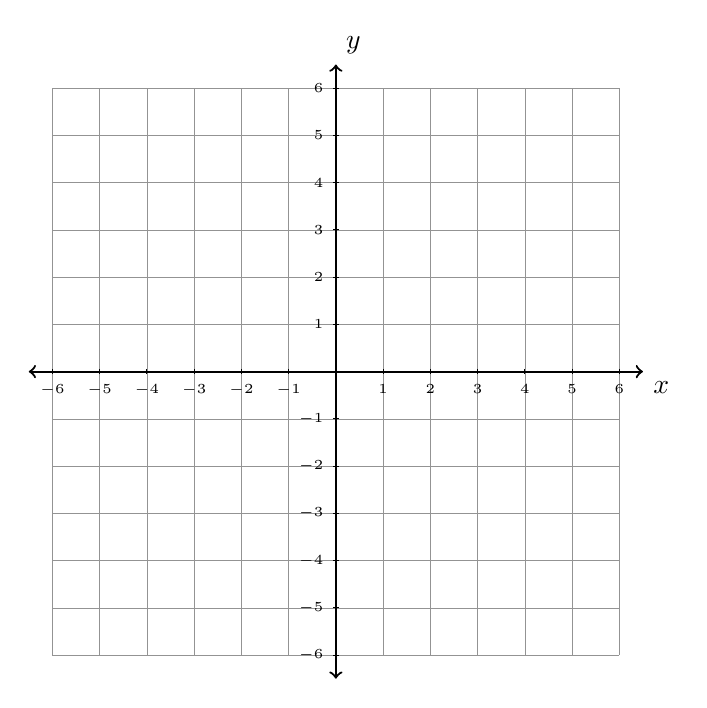
\begin{tikzpicture}[y=.6cm, x=.6cm,font=\sffamily,
	mydot/.style={
    circle,
    fill=white,
    draw,
    outer sep=0pt,
    inner sep=1.5pt
  }]
    %% Add a grid
    \draw[step = 1, gray, very thin,opacity=0.85] (-6, -6) grid (6, 6);
 	%% Draw the axes
	\draw[thick,<->] (-6.5,0) -- coordinate (x axis mid) (6.5,0) node[anchor = north west] {$x$};
    \draw[thick,<->] (0,-6.5) -- coordinate (y axis mid) (0,6.5) node[anchor = south west] {$y$};
    %% Label the y axis
    \foreach \y in {-6,...,-1,1,2,...,6} {
      \draw (1pt, \y) -- (-1pt, \y) node[anchor =  east] {\tiny$\y$};
    }
    %% Label the x axis
    \foreach \x in {-6,...,-1,1,2,...,6} {
      \draw (\x,1pt) -- (\x,-1pt) node[anchor = north] {\tiny$\x$};
    }
    %% Draw the function.
 %   \begin{scope}
 %        \draw[very thick,black] (-3,2) -- (1,1);
 %        \draw[very thick,black] (3.05,1.05) -- (4,3);
    %semi-circle
  %       \draw[very thick, black] (1,1) arc [radius=1, start angle=180, end angle= 5];
     %parabola
     %    \draw[ultra thick, black, domain=-5:0] plot (\x, {(-0.2)*(\x-5)*(\x+5)});
     %dots
     %  \fill[black] (-3, 2) circle[radius=0.5ex];
     %   \fill[black] (1,1) circle[radius=0.5ex];
     %    \fill[black] (4,3) circle[radius=0.5ex];
     %     \draw[very thick, black] (3,1) circle[radius=0.5ex];


   % \end{scope}

    %%\node[above=0.1cm] at (-2,2 )   {\nextXValue};

  \end{tikzpicture}



\columnbreak

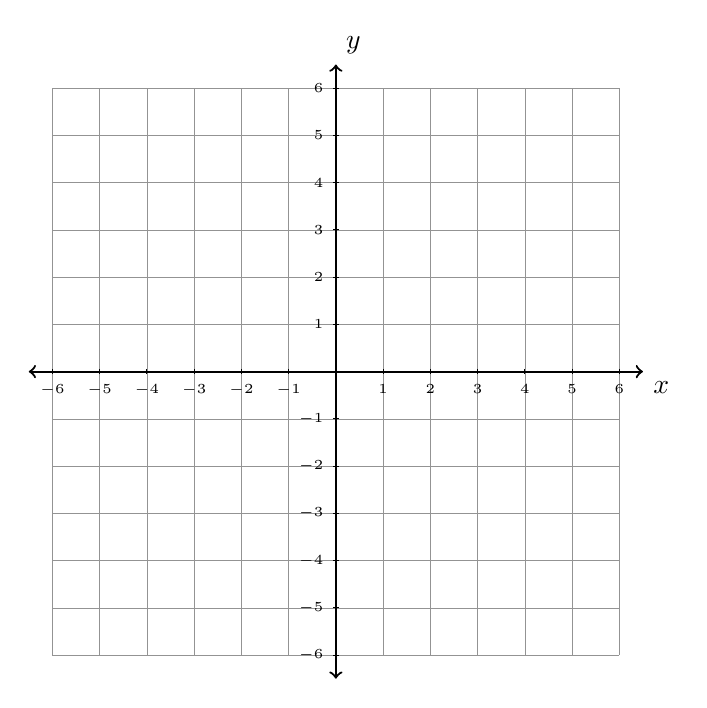
\begin{tikzpicture}[y=.6cm, x=.6cm,font=\sffamily,
	mydot/.style={
    circle,
    fill=white,
    draw,
    outer sep=0pt,
    inner sep=1.5pt
  }]
    %% Add a grid
    \draw[step = 1, gray, very thin,opacity=0.85] (-6, -6) grid (6, 6);
 	%% Draw the axes
	\draw[thick,<->] (-6.5,0) -- coordinate (x axis mid) (6.5,0) node[anchor = north west] {$x$};
    \draw[thick,<->] (0,-6.5) -- coordinate (y axis mid) (0,6.5) node[anchor = south west] {$y$};
    %% Label the y axis
    \foreach \y in {-6,...,-1,1,2,...,6} {
      \draw (1pt, \y) -- (-1pt, \y) node[anchor =  east] {\tiny$\y$};
    }
    %% Label the x axis
    \foreach \x in {-6,...,-1,1,2,...,6} {
      \draw (\x,1pt) -- (\x,-1pt) node[anchor = north] {\tiny$\x$};
    }
    %% Draw the function.
 %   \begin{scope}
 %        \draw[very thick,black] (-3,2) -- (1,1);
 %        \draw[very thick,black] (3.05,1.05) -- (4,3);
    %semi-circle
  %       \draw[very thick, black] (1,1) arc [radius=1, start angle=180, end angle= 5];
     %parabola
     %    \draw[ultra thick, black, domain=-5:0] plot (\x, {(-0.2)*(\x-5)*(\x+5)});
     %dots
     %  \fill[black] (-3, 2) circle[radius=0.5ex];
     %   \fill[black] (1,1) circle[radius=0.5ex];
     %    \fill[black] (4,3) circle[radius=0.5ex];
     %     \draw[very thick, black] (3,1) circle[radius=0.5ex];


   % \end{scope}

    %%\node[above=0.1cm] at (-2,2 )   {\nextXValue};

  \end{tikzpicture}
  

\vspace{1in}


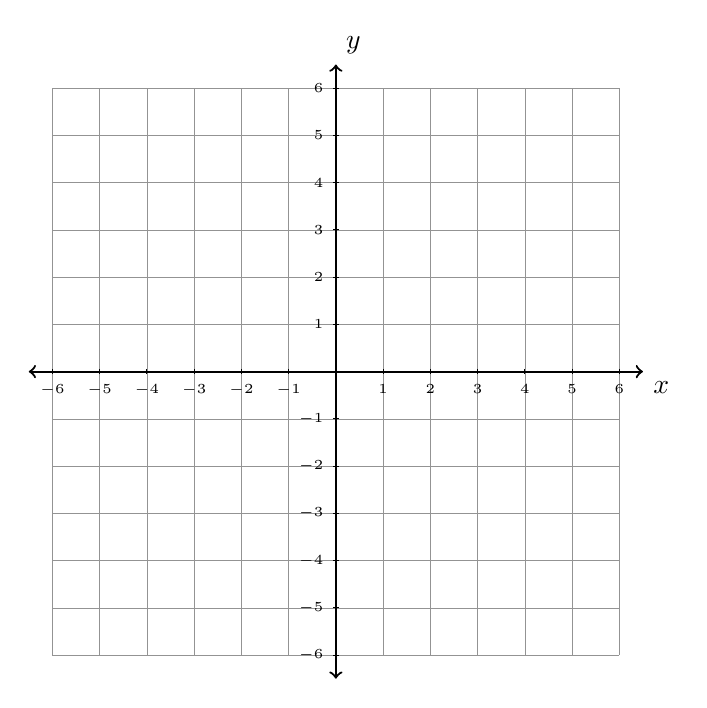
\begin{tikzpicture}[y=.6cm, x=.6cm,font=\sffamily,
	mydot/.style={
    circle,
    fill=white,
    draw,
    outer sep=0pt,
    inner sep=1.5pt
  }]
    %% Add a grid
    \draw[step = 1, gray, very thin,opacity=0.85] (-6, -6) grid (6, 6);
 	%% Draw the axes
	\draw[thick,<->] (-6.5,0) -- coordinate (x axis mid) (6.5,0) node[anchor = north west] {$x$};
    \draw[thick,<->] (0,-6.5) -- coordinate (y axis mid) (0,6.5) node[anchor = south west] {$y$};
    %% Label the y axis
    \foreach \y in {-6,...,-1,1,2,...,6} {
      \draw (1pt, \y) -- (-1pt, \y) node[anchor =  east] {\tiny$\y$};
    }
    %% Label the x axis
    \foreach \x in {-6,...,-1,1,2,...,6} {
      \draw (\x,1pt) -- (\x,-1pt) node[anchor = north] {\tiny$\x$};
    }
    %% Draw the function.
 %   \begin{scope}
 %        \draw[very thick,black] (-3,2) -- (1,1);
 %        \draw[very thick,black] (3.05,1.05) -- (4,3);
    %semi-circle
  %       \draw[very thick, black] (1,1) arc [radius=1, start angle=180, end angle= 5];
     %parabola
     %    \draw[ultra thick, black, domain=-5:0] plot (\x, {(-0.2)*(\x-5)*(\x+5)});
     %dots
     %  \fill[black] (-3, 2) circle[radius=0.5ex];
     %   \fill[black] (1,1) circle[radius=0.5ex];
     %    \fill[black] (4,3) circle[radius=0.5ex];
     %     \draw[very thick, black] (3,1) circle[radius=0.5ex];


   % \end{scope}

    %%\node[above=0.1cm] at (-2,2 )   {\nextXValue};

  \end{tikzpicture}
  
  
\end{multicols}

\clearpage

\item Determine whether or not each relationship below is a function.
  For each relationship that is a function briefly discuss whether or
  not it is a one-to-one function. Briefly explain your reasoning. if
  a function is not one-to-one determine a restriction on the domain
  so that it is one-to-one on the restricted domain.

  \begin{enumerate}
  \item ~ \\
  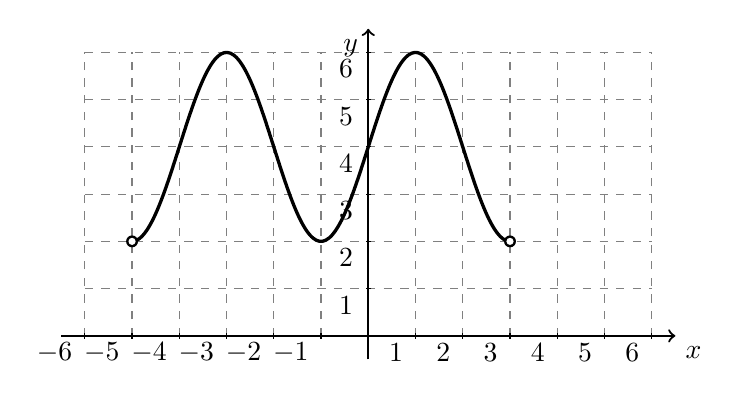
\begin{tikzpicture}[y=0.6cm, x=0.6cm,font=\sffamily]
    %% ticks
    \draw[step = 1, gray,dashed] (-6,0) grid (6,6);
    %% axis
    \draw[thick,->] (-6.5,0) -- coordinate (x axis mid) (6.5,0) node[anchor = north west] {$x$};
    \draw[thick,->] (0,-.5) -- coordinate (y axis mid) (0,6.5) node[anchor = north east] {$y$};
    \foreach \y in {1,2,...,6} {
      \draw (1pt, \y) -- (-1pt, \y) node[yshift=-6,xshift=-1,anchor=east] {$\y$};
    }
    \foreach \x in {-6,-5,...,-1,1,2,...,6} {
      \draw (\x,1pt) -- (\x,-1pt) node[yshift=-5,xshift=-1,anchor=east] {$\x$};
    }

    \begin{scope}
      %\clip(-4,-1) rectangle (8,5);
      \draw[scale=1.0,domain=-4:4,smooth,variable=\x,very thick,black,samples=120] 
           plot ({\x-1},{4+2*sin(deg(pi*\x/2-pi/2))});
      \fill[black] (-5,2) circle [radius=0.5ex];
      \fill[white] (-5,2) circle [radius=0.3ex];
      \fill[black] ( 3,2) circle [radius=0.5ex];
      \fill[white] ( 3,2) circle [radius=0.3ex];
    \end{scope}

  \end{tikzpicture}

  \vfill
  
  \item ~ \\
    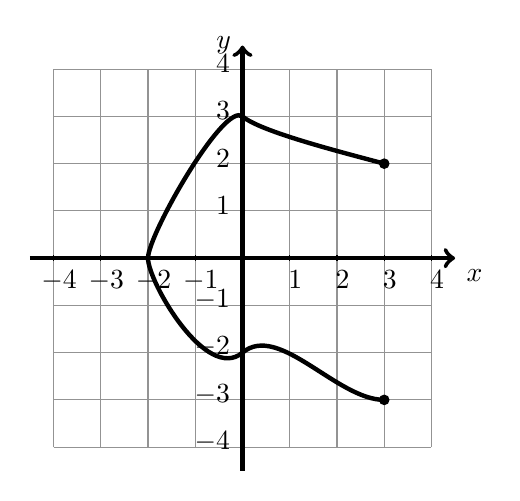
\begin{tikzpicture}[y=0.6cm, x=0.6cm,font=\sffamily]
      \draw[step = 1, gray, thin,opacity=0.85] (-4,-4) grid (4,4);
      \draw[black,ultra thick,->] (-4.5,0) -- (4.5,0) node[anchor=north west] {$x$};
      \draw[black,ultra thick,->] (0,-4.5) -- (0,4.5) node[anchor=east] {$y$};
      \foreach \y in {-4,-3,-2,-1,1,2,3,4} {
        \draw (1pt, \y) -- (-1pt, \y) node[anchor = east,yshift=2] {$\y$};
        \draw (\y,1pt) -- (\y,-1pt) node[anchor = north,xshift=2] {$\y$};
      }
      \draw[ultra thick,black] (3, -3) .. controls +(0:-1) and +(40:1) .. (0, -2)
                    ( 0,-2) .. controls +( 40:-1.0) and +(90:-0.5) .. (-2, 0)
                    (-2, 0) .. controls +( 90:0.5) and +(-40:-0.5) .. (0,3)
                    ( 0, 3) .. controls +(-40:0.5) and +(-15:-1) .. (3, 2);
          \draw[black,fill=black]  (3,-3) circle (0.1);
          \draw[black,fill=black]  (3, 2) circle (0.1);

    \end{tikzpicture}

    \vfill
    
    \item ~ \\
    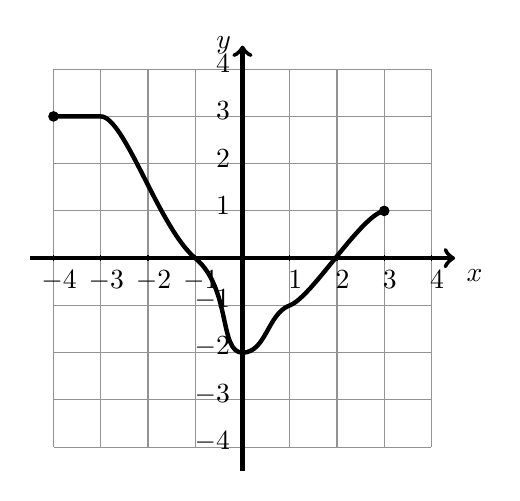
\begin{tikzpicture}[y=0.6cm, x=0.6cm,font=\sffamily]
      \draw[step = 1, gray, thin,opacity=0.85] (-4,-4) grid (4,4);
      \draw[black,ultra thick,->] (-4.5,0) -- (4.5,0) node[anchor=north west] {$x$};
      \draw[black,ultra thick,->] (0,-4.5) -- (0,4.5) node[anchor=east] {$y$};
      \foreach \y in {-4,-3,-2,-1,1,2,3,4} {
        \draw (1pt, \y) -- (-1pt, \y) node[anchor = east,yshift=2] {$\y$};
        \draw (\y,1pt) -- (\y,-1pt) node[anchor = north,xshift=2] {$\y$};
      }
      \draw[ultra thick,black]
                    (-4,3)  .. controls +(0:1) and +(180:0.5) .. (-3,3)
                    (-3, 3) .. controls +(0:0.5) and +(140:1) .. (-1, 0)
                    ( -1,0) .. controls +( 140:-1) and +(180:0.5) .. (0, -2)
                    ( 0, -2) .. controls +(0:0.5) and +(200:0.5) .. (1,-1)
                    ( 1, -1) .. controls +(200:-0.5) and  +(190:0.5) .. (3,1);
          \draw[black,fill=black]  (-4,3) circle (0.1);
          \draw[black,fill=black]  (3, 1) circle (0.1);

    \end{tikzpicture}

    \vfill
    
  \end{enumerate}

\end{enumerate}

\hwTitle{Section 3.1}

\begin{enumerate}
\item The graph of a function, $h$, is given in the plot below, and a
  table is given for all of the values of a function, $g$. Use the
  information in the graph and the table to answer each of the
  questions below. \textbf{If a value does not exist briefly explain
    why.}

  \begin{tabular}{p{0.7\textwidth}p{0.2\textwidth}}
    \begin{minipage}{0.7\linewidth}
      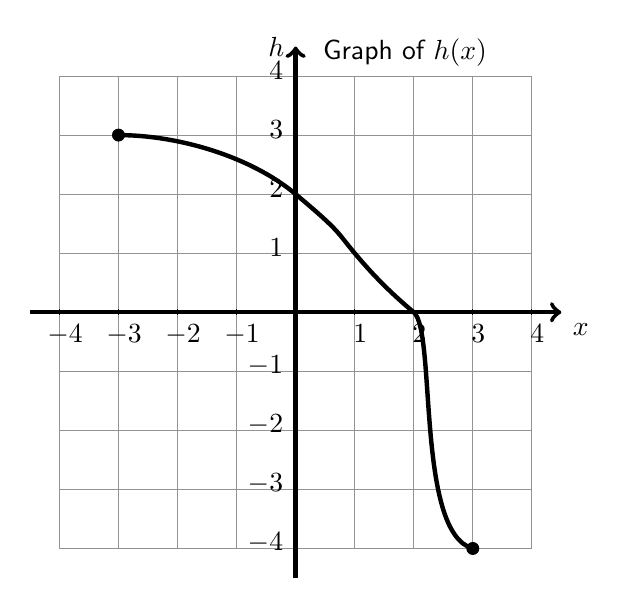
\begin{tikzpicture}[y=0.75cm, x=0.75cm,font=\sffamily]
        \draw[step = 1, gray, thin,opacity=0.85] (-4,-4) grid (4,4);
        \draw[black,ultra thick,->] (-4.5,0) -- (4.5,0) node[anchor=north west] {$x$};
        \draw[black,ultra thick,->] (0,-4.5) -- (0,4.5) node[anchor=east] {$h$};
        \node[black,anchor=south west] at (0.3,4) {Graph of $h(x)$};
        \foreach \y in {-4,-3,-2,-1,1,2,3,4} {
          \draw (1pt, \y) -- (-1pt, \y) node[anchor = east,yshift=2] {$\y$};
          \draw (\y,1pt) -- (\y,-1pt) node[anchor = north,xshift=2] {$\y$};
        }
        %% Draw the function.
        \begin{scope}
          \draw[ultra thick,black] (-3, 3) .. controls +(0:1) and +(-40:-1) .. (0, 2)
                    ( 0, 2) .. controls +(-40:1.0) and +(-50:-0.5) .. (1, 1)
                    ( 1, 1) .. controls +(-50:0.5) and +(-40:-0.5) .. (2,0)
                    ( 2,0) .. controls +(-40:0.5) and +(-15:-1) .. (3, -4);
          \draw[black,fill=black]  (-3,3) circle (0.1);
          \draw[black,fill=black]  (3,-4) circle (0.1);
        \end{scope}
      \end{tikzpicture}
    \end{minipage}
    &
      \begin{minipage}{0.2\linewidth}
        \begin{tabular}{r|r}
          $x$ & $g(x)$ \\ \hline
          0 & 5 \\
          1 & 0 \\
          2 & -3 \\
          3 & 1 \\
          4 & 3 
        \end{tabular}
      \end{minipage}
  \end{tabular}

  \begin{enumerate}
  \item  Is the function $h$ 1-1? (Briefly justify your answer.)
  \item  Determine the value of $g(h(2))$.
  \item  Determine the value of  $h(g(2))$.
  \item  Determine the value of $g^{-1}(h(3))$.
  \item  Determine the value of $g(h^{-1}(3))$.
  \item  Determine the range and domain of $g^{-1}$.
  \item  Determine the range and domain of $h^{-1}$.
  \end{enumerate}

\item The following questions refer to the functions whose graphs are
  given below.x

    \begin{tabular}{p{0.5\textwidth}p{0.5\textwidth}}
    \begin{minipage}{0.5\linewidth}
      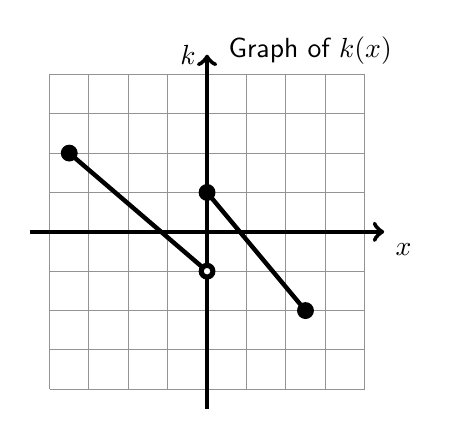
\begin{tikzpicture}[y=0.5cm, x=0.5cm,font=\sffamily]
        \draw[step = 1, gray, thin,opacity=0.85] (-4,-4) grid (4,4);
        \draw[black,ultra thick,->] (-4.5,0) -- (4.5,0) node[anchor=north west] {$x$};
        \draw[black,ultra thick,->] (0,-4.5) -- (0,4.5) node[anchor=east] {$k$};
        \node[black,anchor=south west] at (0.3,4) {Graph of $k(x)$};
        %\foreach \y in {-4,-3,-2,-1,1,2,3,4} {
        %  \draw (1pt, \y) -- (-1pt, \y) node[anchor = east,yshift=2] {$\y$};
        %  \draw (\y,1pt) -- (\y,-1pt) node[anchor = north,xshift=2] {$\y$};
        %}
        %% Draw the function.
        \begin{scope}
          \draw[black,ultra thick] (-3.5,2) -- (0,-1);
          \draw[black,ultra thick] (0,1)    -- (2.5,-2);
          \draw[black,fill=black]  (-3.5,2) circle (0.2);
          \draw[black,fill=black]  (0,-1) circle (0.2);
          \draw[black,fill=white]  (0,-1) circle (0.1);
          \draw[black,fill=black]  (0, 1) circle (0.2);
          \draw[black,fill=black]  (2.5,-2) circle (0.2);
        \end{scope}
      \end{tikzpicture}
    \end{minipage}
    &
      \begin{minipage}{0.5\linewidth}
      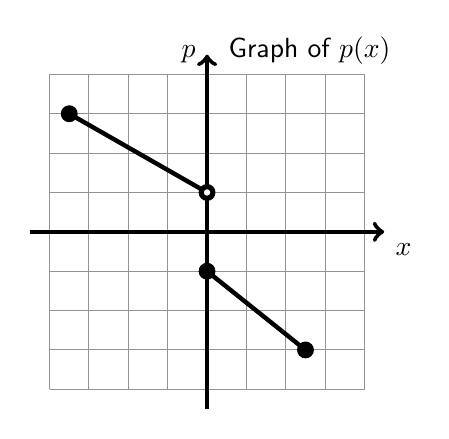
\begin{tikzpicture}[y=0.5cm, x=0.5cm,font=\sffamily]
        \draw[step = 1, gray, thin,opacity=0.85] (-4,-4) grid (4,4);
        \draw[black,ultra thick,->] (-4.5,0) -- (4.5,0) node[anchor=north west] {$x$};
        \draw[black,ultra thick,->] (0,-4.5) -- (0,4.5) node[anchor=east] {$p$};
        \node[black,anchor=south west] at (0.3,4) {Graph of $p(x)$};
        %\foreach \y in {-4,-3,-2,-1,1,2,3,4} {
        %  \draw (1pt, \y) -- (-1pt, \y) node[anchor = east,yshift=2] {$\y$};
        %  \draw (\y,1pt) -- (\y,-1pt) node[anchor = north,xshift=2] {$\y$};
        %}
        %% Draw the function.
        \begin{scope}
          \draw[black,ultra thick] (-3.5,3) -- (0,1);
          \draw[black,ultra thick] (0,-1)    -- (2.5,-3);
          \draw[black,fill=black]  (-3.5,3) circle (0.2);
          \draw[black,fill=black]  (0,1) circle (0.2);
          \draw[black,fill=white]  (0,1) circle (0.1);
          \draw[black,fill=black]  (0,-1) circle (0.2);
          \draw[black,fill=black]  (2.5,-3) circle (0.2);
        \end{scope}
      \end{tikzpicture}
      \end{minipage}
    \end{tabular}

    \begin{enumerate}
    \item Determine the domain of $k(x)$ and determine the set of
      values of $x$ over which the function is decreasing. Is the
      function, $k(x)$, one-to-one? (Briefly justify your reasoning.)
    \item Determine the domain of $p(x)$ and determine the set of
      values of $x$ over which the function is decreasing. Is the
      function, $p(x)$, one-to-one? (Briefly justify your reasoning.)
    \item Are $k(x)$ and $p(x)$ strictly decreasing functions? If a
      function is strictly decreasing is the function one-to-one?
      (Briefly justify your reasoning.)
    \end{enumerate}

  \item The graph of a function is given below. Determine whether or
    not an inverse for the function exists. If not determine a
    restriction on the domain so that the function is invertable on
    your restricted domain. Your restricted domain should allow you to
    invert the function for any value of $y$ in the range of the
    original function.

      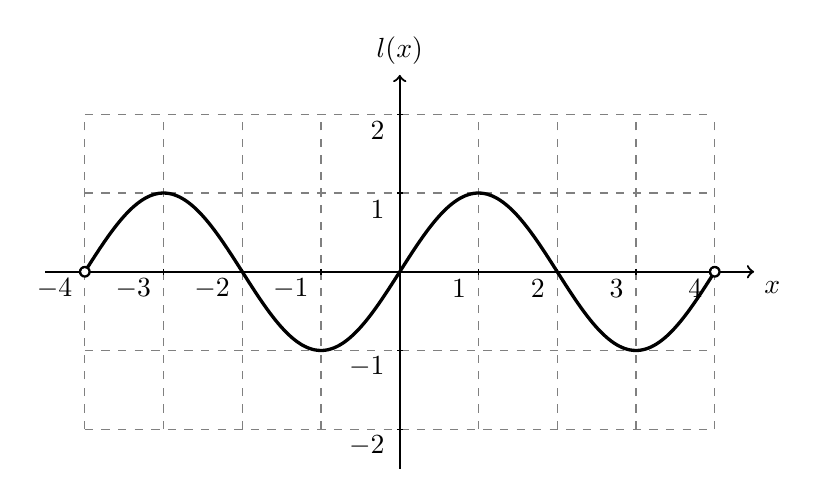
\begin{tikzpicture}[y=1.0cm, x=1.0cm,font=\sffamily]
    %% ticks
    \draw[step = 1, gray,dashed] (-4,-2) grid (4,2);
    %% axis
    \draw[thick,->] (-4.5,0) -- coordinate (x axis mid) (4.5,0) node[anchor = north west] {$x$};
    \draw[thick,->] (0,-2.5) -- coordinate (y axis mid) (0,2.5) node[anchor = south] {$l(x)$};
    \foreach \y in {-2,-1,1,2} {
      \draw (1pt, \y) -- (-1pt, \y) node[yshift=-6,xshift=-1,anchor=east] {$\y$};
    }
    \foreach \x in {-4,-3,...,-1,1,2,...,4} {
      \draw (\x,1pt) -- (\x,-1pt) node[yshift=-5,xshift=-1,anchor=east] {$\x$};
    }

    \begin{scope}
      %\clip(-4,-1) rectangle (8,5);
      \draw[scale=1.0,domain=-4:4,smooth,variable=\x,very thick,black,samples=120] 
           plot ({\x},{sin(deg(pi*\x/2))});
      \fill[black] (-4,0) circle [radius=0.5ex];
      \fill[white] (-4,0) circle [radius=0.3ex];
      \fill[black] ( 4,0) circle [radius=0.5ex];
      \fill[white] ( 4,0) circle [radius=0.3ex];
    \end{scope}

  \end{tikzpicture}

\item The equation for a function, $j(x)$, is given below, and a table
  is given for all of the values of a function, $v(x)$. Use the
  formula and the table to answer each of the questions
  below. \textbf{If a value does not exist briefly explain why.}

  \begin{tabular}{p{0.3\textwidth}p{0.3\textwidth}}
    \begin{minipage}{0.3\linewidth}
      \begin{eqnarray*}
        j(x) & = & |x|,
      \end{eqnarray*}
    \end{minipage}
    &
      \begin{minipage}{0.3\linewidth}
        \begin{tabular}{r|r}
          $x$ & $v(x)$ \\ \hline
          0 & 10 \\
          1 &  8 \\
          2 &  4 \\
          3 &  0 \\
          4 & -2
        \end{tabular}
      \end{minipage}
  \end{tabular}

  \begin{enumerate}
  \item  Is the function $j$ 1-1? (Briefly justify your answer.)
  \item  Is the function $v$ 1-1? (Briefly justify your answer.)
  \item  Determine the value of $j(v(2))$.
  \item  Determine the value of  $v(j(-2))$.
  \item  Determine the value of $v^{-1}(j(-3))$.
  \item  Determine the value of $v(j^{-1}(-3))$.
  \item  Determine the range and domain of $v^{-1}$.
  \end{enumerate}


\end{enumerate}


